\section{Prompts}
\label{app:prompts}

\paragraph{Selector.} The \qss{} selector and all lightweight selectors receive the following system instruction, followed by the index (or the prefiltered index), optionally the block of resolved earlier questions, and the question. The output is constrained to the JSON schema \texttt{\{"rounds": [string]\}}.

\begin{quote}\small
You are the retrieval step of a personal assistant's long-term memory. You get a compact index of the user's entire conversation history (one line per round; images are summarised in a few words) and a question. Choose the rounds that must be opened in full (with their original images) to answer the question. Include EVERY round that may hold needed evidence, especially ALL members of any group the question refers to (e.g. all ads of a brand, every scene of an episode, all versions of a screen over time), not just the best match. Include rounds that define labels the question uses (episode/arc names, `first', `later', `updated'). Image summaries are lossy: when unsure whether an image is relevant, include it. Order by importance. Return JSON with the key ``rounds'' and at most 40 ids.
\end{quote}

\paragraph{Controls.} The ranking control receives the same candidate index lines with the instruction to rank all candidate rounds from most to least useful for answering the question and to return all identifiers in order. The recall-oriented ranking control receives the selector instruction above with only its output changed: it ranks all candidate rounds by how likely they must be opened, ranking first every round that may hold needed evidence, all members of any group that the question refers to, rounds that define labels used by the question, and rounds whose image summary is too coarse to rule them out. The dynamic cut-off control receives the same lines with the instruction to rate every candidate from 0 (not relevant) to 3 (contains needed evidence) and returns a JSON map from round identifiers to grades; rounds graded 2 or 3 are kept. Selectors from other families receive the identical selector instruction through OpenRouter with JSON output.

\paragraph{Resolution write-back.} Earlier resolutions are appended after the index as lines that pair an earlier question with its selected round identifiers, under the header ``Resolved earlier questions from this user (the rounds that were opened to answer them; the labels they use may refer to the same items as the current question)''.

\paragraph{Reader.} All conditions with the same reader share one system instruction. It asks the reader to ground every answer in the provided history and images, to prefer the most recent evidence when information conflicts, to inspect images carefully, to state when information is absent, to name images the way the conversation described them, and to answer concisely. The last rule was introduced before any reported run to stop the reader from answering with bracketed image identifiers, and its example phrase (``the provisional busy-day trend'') coincides with the gold answer of two MemEye questions. Because the instruction is identical in every condition, it cannot favor one method; excluding the two questions changes the main differences by at most 0.001 (\qss{} minus top-40 retrieval: $+0.054$ $[+0.009, +0.098]$ with the lightweight reader and $+0.056$ $[+0.022, +0.090]$ with the strong reader and the index as context).

\paragraph{Judges.} On MemEye, the judge uses the official rubric, which scores an answer in $\{0, 0.25, 0.5, 0.75, 1\}$ against the reference answer. On MemLens, the judge uses the official type-specific prompts of the benchmark (binary scores) without modification.

\section{Additional Results}
\label{app:results}

\paragraph{Scenario-level uncertainty on MemEye.} Table~\ref{tab:cluster} repeats the main MemEye contrasts under a two-stage bootstrap that resamples the eight scenario histories and then questions within them.

\begin{table}[h]
\centering
\caption{Question-level and scenario-level 95\% bootstrap intervals for the main MemEye contrasts, with the number of scenarios (out of 8) whose mean difference is positive and a Wilcoxon signed-rank test over the eight scenario means.}
\label{tab:cluster}
\small
\resizebox{\linewidth}{!}{%
\begin{tabular}{lcccrr}
\toprule
Contrast & Mean & Question-level CI & Scenario-level CI & Scenarios $>0$ & Wilcoxon $p$ \\
\midrule
Lightweight reader: \qss{} $-$ RAG@40 & $+0.053$ & $[+0.009, +0.098]$ & $[-0.014, +0.120]$ & 6/8 & 0.078 \\
Lightweight reader with thinking: \qss{} $-$ RAG@40 & $+0.045$ & $[+0.003, +0.086]$ & $[-0.005, +0.095]$ & 6/8 & 0.031 \\
Lightweight reader: consensus $-$ RAG@40 & $+0.028$ & $[-0.015, +0.071]$ & $[-0.038, +0.093]$ & 5/8 & 0.250 \\
Strong reader: \qss{} with index $-$ RAG@40 & $+0.055$ & $[+0.021, +0.089]$ & $[+0.004, +0.126]$ & 6/8 & 0.031 \\
Strong reader: \qss{} $-$ RAG@40 & $+0.020$ & $[-0.014, +0.055]$ & $[-0.030, +0.073]$ & 6/8 & 0.219 \\
Strong reader: \qss{} with index $-$ full context & $-0.024$ & $[-0.050, +0.002]$ & $[-0.061, +0.022]$ & 1/8 & 0.438 \\
FSR: \qss{} $-$ cosine of the same size & $+0.364$ & $[+0.310, +0.418]$ & $[+0.221, +0.551]$ & 8/8 & 0.008 \\
FSR: \qss{} ($P{=}100$) $-$ ranking control & $+0.059$ & $[+0.032, +0.089]$ & $[+0.008, +0.111]$ & 5/8 & 0.062 \\
\bottomrule
\end{tabular}}
\end{table}

\paragraph{Independent judge on MemEye.} Qwen3-VL-235B-A22B re-scored the main MemEye conditions with the same rubric. Its scores are lower than those of the primary judge, exact agreement ranges from 0.69 to 0.87 per condition, and every ordering is preserved: for the lightweight reader, \qss{} 0.514, annotated evidence 0.520, full context 0.469, and RAG@40 0.457; for the strong reader, full context 0.758, \qss{} with index 0.739, \qss{} 0.701, and RAG@40 0.695.

\paragraph{Scale and a second benchmark.} Table~\ref{tab:robust} and Figure~\ref{fig:scale} report MemEye histories enlarged by 1,000 distractor images and the 903-question Mem-Gallery subset. On enlarged histories, full-context reading with the lightweight reader drops from 0.495 to 0.368, while \qss{} stays at 0.538 ($+0.067$ $[+0.024, +0.111]$ over top-40 retrieval). On Mem-Gallery, \qss{} with the lightweight reader gains $+0.035$ $[+0.015, +0.056]$ over full context and $+0.013$ $[-0.006, +0.032]$ over top-40 retrieval, and the strong reader shows no difference among the three; full-context reading without any visual information still reaches 0.892 on a fixed half of the subset (451 questions).

\begin{table}[h]
\centering
\caption{Robustness on MemEye histories enlarged by 1,000 distractor images (MemEye+1k, 371 questions) and on Mem-Gallery (903 questions). \qss{} uses a cosine prefilter of 200 rounds on MemEye+1k. $^\dagger$Measured on a fixed 100-question subset that is easier than average for retrieval.}
\label{tab:robust}
\small
\begin{tabular}{llccccc}
\toprule
Setting & Reader & FC & RAG@20 & RAG@40 & Lightweight selector & \qss{} \\
\midrule
MemEye (original) & 2.5-flash-lite & 0.495 & 0.471 & 0.488 & 0.516 & \textbf{0.541} \\
MemEye+1k & 2.5-flash-lite & 0.368 & 0.451 & 0.471 & 0.493 & \textbf{0.538} \\
MemEye+1k & 3.8-flash & 0.848$^\dagger$ & -- & 0.730 & -- & 0.764 \\
Mem-Gallery & 2.5-flash-lite & 0.817 & -- & 0.839 & 0.839 & \textbf{0.852} \\
Mem-Gallery & 3.8-flash & \textbf{0.917} & -- & 0.912 & -- & 0.908 \\
\bottomrule
\end{tabular}
\end{table}

\begin{figure}[h]
\centering
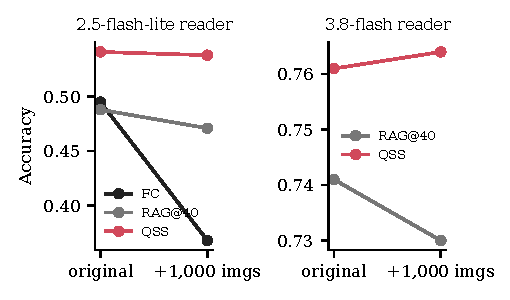
\includegraphics[width=0.5\linewidth]{figures/scale.pdf}
\caption{Accuracy of full context, RAG@40, and \qss{} on the original MemEye histories and on histories enlarged by 1,000 distractor images (32-fold more rounds), for the lightweight reader (left) and the strong reader (right; full context omitted, see Table~\ref{tab:robust}).}
\label{fig:scale}
\end{figure}

\paragraph{MemLens by question type.} Table~\ref{tab:memlens_type} breaks the held-out accuracy of the lightweight reader down by question type.

\begin{table}[h]
\centering
\caption{MemLens-32k accuracy of the lightweight reader by question type (official judge; 246, 194, 143, and 116 questions).}
\label{tab:memlens_type}
\small
\begin{tabular}{lcccc}
\toprule
Method & Information extraction & Temporal reasoning & Multi-session reasoning & Knowledge update \\
\midrule
Full context & 0.577 & 0.557 & 0.182 & 0.353 \\
RAG@40 & 0.598 & 0.552 & 0.189 & 0.431 \\
Annotated evidence & 0.634 & 0.552 & 0.224 & 0.448 \\
\qss{}, frozen design & 0.626 & 0.521 & 0.252 & 0.405 \\
\qss{}, 600-character snippets & 0.634 & 0.577 & 0.266 & 0.388 \\
Dynamic cut-off control & 0.630 & 0.505 & 0.203 & 0.422 \\
\bottomrule
\end{tabular}
\end{table}

\paragraph{MemLens gold rounds.} MemLens annotates answer sessions and flags the user turns that state the evidence; the evidence images are stored in a separate needle folder and usually appear in a different turn of the same session than the flagged text. We therefore define the gold rounds of a question as the rounds of its answer sessions that contain a flagged turn or a needle image (5.9 per question; 4.1 with an image). Every question has at least one gold round with an image.

\paragraph{Reader dependence.} Table~\ref{tab:reader} compares full context with focused evidence for three readers on MemEye. Only the strongest reader benefits from the full history; for the two lighter readers, the annotated evidence is the most accurate input.

\begin{table}[h]
\centering
\caption{Accuracy on MemEye (371 questions) by reader and input. Images at the standard resolution of each reader; no thinking for \texttt{gemini-2.5-flash-lite}.}
\label{tab:reader}
\small
\begin{tabular}{lcccc}
\toprule
Reader & Full context & RAG@10 & RAG@40 & Annotated evidence \\
\midrule
\texttt{gemini-3.8-flash} & 0.819 & 0.689 & 0.741 & 0.746 \\
\texttt{gemini-3.1-flash-lite} & 0.639 & 0.601 & 0.612 & 0.694 \\
\texttt{gemini-2.5-flash-lite} & 0.495 & 0.446 & 0.488 & 0.539 \\
\bottomrule
\end{tabular}
\end{table}

\paragraph{Retrieval keys.} Table~\ref{tab:keys} reports the retrieval keys compared in Section~\ref{sec:prelim}.

\begin{table}[h]
\centering
\caption{Retrieval keys on MemEye: fraction of gold evidence rounds among the top 10 (371 questions).}
\label{tab:keys}
\small
\begin{tabular}{lc}
\toprule
Round key embedded with \texttt{gemini-embedding-2} & Coverage@10 \\
\midrule
Image only & 0.300 \\
Dialogue text only & 0.538 \\
Dialogue text and images in one embedding & 0.671 \\
Dialogue text + dense caption & 0.774 \\
Dialogue text + short caption & 0.774 \\
\bottomrule
\end{tabular}
\end{table}

\paragraph{Scale and determinism.} With the strong reader, the apparent drop of top-40 retrieval from 0.820 to 0.762 on a 100-question subset at +1,000 images is not attributable to retrieval: 62 of the 100 questions retrieved exactly the same rounds at both scales, and re-running the original prompts with a second seed moved the same 62 questions by a similar amount. We therefore report full-set recall and the 371-question comparisons at scale. The lightweight reader is deterministic at temperature 0 without thinking, so its comparisons contain no decoding noise; the strong reader varies between seeds by 0.01--0.04 on condition means. The strong selector also varies between draws: only about half of the selected sets are identical across two draws on MemEye, and Section~\ref{sec:rq6} reports the resulting variation of end-to-end accuracy.

\paragraph{Index visibility and gold definitions.} Table~\ref{tab:visibility} reports the two analyses of Section~\ref{sec:rq3}. The upper part manipulates index visibility on MemEye: every content word of the question is replaced by a placeholder with probability $p$ in the index lines of all rounds, gold and non-gold alike, deterministically per question, round, and word, while the reader still receives the raw rounds. The lower part recomputes full-set recall on MemLens under three alternative gold definitions: the rounds with an evidence turn, the rounds with an evidence image, and the coverage of the answer sessions (at least one opened round per answer session).

\begin{table}[h]
\centering
\caption{Index visibility and gold definitions. Upper part: MemEye (371 questions), \qss{} with the strong selector and the lightweight reader with thinking; $\Delta$ is the paired difference from $p{=}0$ with a 95\% bootstrap interval. Lower part: full-set recall on MemLens-32k (699 questions) under alternative gold definitions; ``cosine'' opens the same number of rounds as the selector in the row above it.}
\label{tab:visibility}
\small
\resizebox{\linewidth}{!}{%
\begin{tabular}{lcccc}
\toprule
\multicolumn{5}{l}{\textit{Masking question words in the index (MemEye)}} \\
Masking probability $p$ & Rounds & FSR & $\Delta$ FSR & Accuracy ($\Delta$) \\
\midrule
0 & 7.3 & 0.903 & -- & 0.597 \\
0.5 & 8.2 & 0.879 & $-0.024$ $[-0.057, +0.008]$ & 0.604 ($+0.007$ $[-0.024, +0.038]$) \\
1.0 & 8.5 & 0.814 & $-0.089$ $[-0.124, -0.054]$ & 0.511 ($-0.086$ $[-0.127, -0.045]$) \\
\midrule
\multicolumn{5}{l}{\textit{Full-set recall under alternative gold definitions (MemLens-32k)}} \\
Retriever (rounds) & Derived gold & Evidence-turn rounds & Evidence-image rounds & Answer sessions covered \\
\midrule
\qss{}, 200 characters (6.1) & 0.375 & 0.614 & 0.251 & 0.687 \\
\quad cosine, same size & 0.176 & 0.385 & 0.106 & 0.554 \\
\qss{}, 600 characters (3.9) & 0.286 & 0.828 & 0.133 & 0.828 \\
\quad cosine, same size & 0.127 & 0.320 & 0.052 & 0.441 \\
Cosine top-40 (40) & 0.645 & 0.881 & 0.576 & 0.997 \\
\bottomrule
\end{tabular}}
\end{table}

\paragraph{The VGS gate.} Table~\ref{tab:gate} splits the registered MemLens test of Section~\ref{sec:rq5} at the threshold of the visibility estimate. Across the 699 MemLens questions, $\hat{v}(q)$ correlates with the oracle index visibility computed from the gold rounds (Spearman 0.48, AUC 0.75 for an oracle visibility of at least 0.5; means 0.427 and 0.430). By quartile of $\hat{v}(q)$ on the test part, the notes path gains $+0.026$, $+0.128$, $+0.052$, and $+0.009$ over plain \qss{}: the gain is largest at low but not minimal visibility, where the selector still finds part of the set, and it vanishes at high visibility.

\begin{table}[h]
\centering
\caption{The VGS gate on the registered MemLens test part (466 questions, lightweight reader). The last column gives the paired difference between VGS and RAG@40 with a 95\% bootstrap interval.}
\label{tab:gate}
\small
\begin{tabular}{lrccccc}
\toprule
Path & $n$ & RAG@40 & \qss{}, 200 & \qss{}, 600 & \qss{}, 600 + notes & VGS $-$ RAG@40 \\
\midrule
$\hat{v}(q)\ge0.7$ & 59 & 0.559 & 0.542 & 0.542 & 0.542 & $-0.017$ $[-0.136, +0.085]$ \\
$\hat{v}(q)<0.7$ & 407 & 0.452 & 0.474 & 0.469 & 0.536 & $+0.084$ $[+0.042, +0.125]$ \\
All & 466 & 0.466 & 0.483 & 0.479 & 0.536 & $+0.071$ $[+0.032, +0.109]$ \\
\bottomrule
\end{tabular}
\end{table}

\paragraph{Visual and text-only questions.} To test whether the gains of the set path come from questions that need images, a question-only classifier (\texttt{gemini-2.5-flash-lite}, from the question text alone) marks each question as visual or text-only. Table~\ref{tab:visualq} compares the set path with RAG@40 on both groups for the lightweight reader; the set path is \qss{} on MemEye and Mem-Gallery and VGS on MemLens and WorldMemArena (corrected run).

\begin{table}[h]
\centering
\caption{Set path minus RAG@40 for questions classified as visual or text-only (lightweight reader; paired differences with 95\% bootstrap intervals).}
\label{tab:visualq}
\small
\begin{tabular}{lcrr}
\toprule
Benchmark & Visual share & Visual questions & Text-only questions \\
\midrule
MemEye & 0.54 & $+0.039$ $[-0.021, +0.097]$ & $+0.071$ $[+0.006, +0.137]$ \\
MemLens test & 0.35 & $+0.062$ $[+0.000, +0.130]$ & $+0.075$ $[+0.026, +0.125]$ \\
Mem-Gallery & 0.44 & $+0.018$ $[-0.006, +0.042]$ & $+0.010$ $[-0.018, +0.037]$ \\
WorldMemArena & 0.28 & $+0.020$ $[-0.012, +0.052]$ & $+0.003$ $[-0.018, +0.024]$ \\
\bottomrule
\end{tabular}
\end{table}

\paragraph{Compact index.} Table~\ref{tab:compact} reports the selection results behind the compact index of Section~\ref{sec:rq6}. Dropping the assistant snippet removes about a fifth of the input with almost no loss of full-set recall, short identifiers remove another fifth at a small loss, and together the three changes let 600 characters of a long MemLens message fit into fewer tokens than the original 200-character lines (4,026 against 7,166 tokens). End to end, the lightweight reader with thinking reaches 0.597 with the original index and 0.608, 0.596, and 0.600 with the three compact variants on MemEye, and the low-visibility path of VGS reaches 0.562 with both the original and the compact 600-character index on the MemLens development part, whereas a compact 200-character index reaches only 0.515 there.

\begin{table}[h]
\centering
\caption{Selection with compact indexes (\texttt{gemini-3.8-flash} selector). ``No assistant'' drops the assistant snippet, ``short ids'' lists rounds by positional identifiers under one header per session, and ``telegraph'' removes function words from the user text before truncation. MemEye+1k uses a cosine prefilter of $P$ rounds.}
\label{tab:compact}
\small
\begin{tabular}{llrccr}
\toprule
Data & Index & Rounds & FSR & FSR, $\ge$4 gold rounds & Input tokens \\
\midrule
\multirow{5}{*}{MemEye (371 q)} & Original & 7.3 & 0.903 & 0.872 & 11,286 \\
 & No assistant & 7.3 & 0.900 & 0.849 & 8,976 \\
 & No assistant + telegraph & 6.8 & 0.887 & 0.767 & 8,115 \\
 & No assistant + short ids & 7.3 & 0.881 & 0.802 & 6,658 \\
 & All three & 7.2 & 0.876 & 0.791 & 5,797 \\
\midrule
\multirow{4}{*}{MemLens dev (233 q)} & Original, 200 characters & 6.1 & 0.382 & 0.064 & 7,166 \\
 & All three, 200 characters & 6.1 & 0.361 & 0.032 & 3,202 \\
 & Original, 600 characters & 4.0 & 0.292 & 0.064 & 9,328 \\
 & All three, 600 characters & 4.0 & 0.266 & 0.040 & 4,026 \\
\midrule
\multirow{3}{*}{MemEye+1k (371 q)} & Original, $P{=}200$ & 10.7 & 0.914 & 0.802 & 16,791 \\
 & No assistant + telegraph, $P{=}200$ & 11.0 & 0.922 & 0.814 & 10,669 \\
 & No assistant + telegraph, $P{=}320$ & 10.8 & 0.919 & 0.826 & 16,173 \\
\bottomrule
\end{tabular}
\end{table}

\paragraph{Set-aware router.}
\label{app:router}
The router labels a question as multi-item from its text alone; it sees neither the history nor any annotation. It labels 54.7\% of the MemEye questions, 28.8\% of the MemLens questions, and 10.7\% of the Mem-Gallery questions as multi-item. A post hoc comparison with information that the router did not use shows where its labels agree with the evidence and where they do not. On MemEye, it labels 15\% of the questions with one gold round, 72\% of those with two or three, and 77\% of those with four or more as multi-item. On MemLens, it labels all arithmetic, duration-comparison, and ordering questions as multi-item and 1--8\% of the information-extraction and knowledge-update questions, but only 2\% of the counting questions, whose wording often reads like a count within one scene although the answer accumulates items across sessions. Routing therefore gives up part of the gain of set selection on such questions.

\section{Reader-Driven Zooming and Caption Content}
\label{app:zoom}

Three further ideas are often proposed for multimodal memory: letting the reader inspect selected images at higher resolution, storing images as captions written by a stronger model, and extracting question-specific notes from each image before answering. For zooming, the reader first sees the context at standard resolution and requests up to three zoomed crops, each defined by an image identifier and a bounding box; the second pass reuses the baseline prompt when no zoom is requested. A forced variant requires one to three zooms, and a blind control adds three fixed tiles of the image most similar to the question. Table~\ref{tab:zoom} lists all conditions.

\begin{table}[h]
\centering
\caption{Reader-driven zooming (MemEye, 371 questions). ``Reader-chosen'' lets the reader decide whether and where to zoom; ``forced'' requires one to three zooms; ``blind'' adds three fixed tiles of the image most similar to the question.}
\label{tab:zoom}
\small
\begin{tabular}{llcccc}
\toprule
Reader & Evidence & No zoom & Reader-chosen & Forced & Blind \\
\midrule
2.5-flash-lite & Annotated evidence & 0.539 & 0.552 & 0.551 & 0.561 \\
2.5-flash-lite & \qss{} set (7.3 rounds) & 0.541 & 0.539 & 0.557 & 0.523 \\
2.5-flash-lite & Full context & 0.495 & -- & 0.517 & -- \\
3.8-flash & Annotated evidence & 0.746 & -- & 0.777 & 0.725 \\
3.8-flash & Full context (crops appended) & 0.819 & 0.790 & -- & -- \\
3.8-flash & Full context (in-place upgrade) & 0.819 & 0.803 & -- & -- \\
\bottomrule
\end{tabular}
\end{table}

With the strong reader, reader-driven zooming lowers full-context accuracy on MemEye from 0.819 to 0.790, a paired difference of $-0.029$ $[-0.056, -0.002]$, and an in-place upgrade of the zoomed image does not help either ($-0.017$ $[-0.042, +0.009]$). With the lightweight reader on annotated evidence, reader-chosen zooms (0.552) and forced zooms (0.551) do not exceed the blind control (0.561), so the modest improvement over no zoom (0.539) comes from the added pixels rather than from where the reader looks. Dense captions in place of images lower full-context accuracy for both readers (0.779 against 0.819 and 0.474 against 0.495), and adding them next to the images of a \qss{} set does not help (0.526 against 0.541). A map-reduce reader that writes a note per image produces inconsistent effects across the two scenario halves ($+0.000$ and $+0.097$ over top-10 retrieval).

On MemEye, fine detail is therefore rarely the bottleneck for current readers: low resolution matches high resolution in full context, and zooming cannot replace locating the right images, which is the problem that set selection addresses. The per-member notes of VGS differ from this map-reduce reader in two respects that RQ5 tests: they are written only for the members of a selected set, and the reader keeps the raw rounds next to them.

\section{Cost Model}
\label{app:cost}

Costs use list prices per million tokens: \texttt{gemini-3.8-flash} \$0.75 input, \$0.075 cached input, \$3.75 output (including thinking); \texttt{gemini-2.5-flash-lite} \$0.10, \$0.01, and \$0.40; \texttt{gemini-embedding-2} \$0.20 for text and \$0.45 for images. Measured costs use the cached-token counts reported by the API. Our selection runs issued questions concurrently without warming the cache, so only 39\% of the input tokens of strong selection calls were cached. The warm-cache estimate recomputes every question from its logged token counts: the selection call bills the index at the cached rate and the question (about 150 tokens) and the output at full rates, and the index-as-context variant also bills the index part of its reading call at the cached rate. Table~\ref{tab:cost} gives measured, uncached, and warm-cache costs. The later runs with an explicit context cache (Section~\ref{sec:rq6}) measure these warm-cache costs directly: \$7.04 for the strong reader with the index as context (estimate \$6.80), \$2.58 for the lightweight reader with thinking (estimate \$2.39), and \$2.32 to \$2.36 for the lightweight reader without thinking (estimate \$2.20), including the creation and storage of the caches. Top-$k$ retrieval and \qss{} sets cannot be cached across questions because their content differs per question, whereas full-context reading shares the history prefix and was 84--87\% cached in our runs. Writing the index costs one caption per image (about \$0.003 per image for a dense caption and \$0.001 for a short caption with \texttt{gemini-3.8-flash}) and one embedding per round; the predicted aliases of Table~\ref{tab:ablate} cost \$0.21 for all of MemEye.

\begin{table}[h]
\centering
\caption{Cost of \qss{} per 1,000 MemEye questions under three caching assumptions for the static index. References (measured): strong reader RAG@40 \$10.00, RAG@10 \$4.71, full context \$8.97; lightweight reader RAG@40 \$0.86, full context \$0.37.}
\label{tab:cost}
\small
\begin{tabular}{lcccc}
\toprule
Pipeline & Accuracy & Measured & Index uncached & Index cached \\
\midrule
Strong reader, \qss{} & 0.761 & 10.27 & 13.32 & 5.80 \\
Strong reader, \qss{}, index as context & 0.796 & 15.70 & 21.83 & 6.80 \\
Lightweight reader, \qss{} & 0.541 & 6.73 & 9.71 & 2.20 \\
Lightweight reader with thinking, \qss{} & 0.597 & 6.97 & 9.91 & 2.39 \\
\bottomrule
\end{tabular}
\end{table}

\section{Reproducibility}
\label{app:repro}

All code, per-question outputs (retrieved rounds, prediction, judge score and rationale, token usage), and decision logs are in the project repository. \nolinkurl{src/mm2.py} implements the index, \qss{}, the prefilter, the ranking control, the lightweight selectors, resolution write-back, and the zoom protocols; \nolinkurl{scripts/select_eval.py} runs selection-only evaluations; \nolinkurl{scripts/rank_control.py} runs the ranking control; \nolinkurl{scripts/run_mm2.py} runs end-to-end conditions of the form \nolinkurl{selector|reader-mode}; \nolinkurl{scripts/make_tables_p2.py}, \nolinkurl{scripts/analyze_memlens.py}, \nolinkurl{scripts/cluster_stats.py}, and \nolinkurl{scripts/make_figures.py} regenerate the tables and figures from the stored outputs without API calls; \nolinkurl{src/data_memlens.py} loads MemLens, and the registrations of the held-out evaluations (P4-D2, P5-D8, P6-D4, and P7-D1) are recorded in \nolinkurl{notes/RESEARCH_LOG.md} before their first runs. \nolinkurl{scripts/gate_eval.py} combines the paths of VGS, \nolinkurl{scripts/setness.py} writes the router labels, \nolinkurl{scripts/route_eval.py} evaluates routing, and \nolinkurl{scripts/p6_memeye_table.py}, \nolinkurl{scripts/p6_confirm.py}, \nolinkurl{scripts/p7_confirm.py}, and \nolinkurl{scripts/pool_scale.py} produce the results of RQ6; the options \nolinkurl{--xcache} and \nolinkurl{--compact} of \nolinkurl{scripts/run_mm2.py} enable the explicit context cache and the compact index. \nolinkurl{src/data_wma.py} loads WorldMemArena, \nolinkurl{scripts/p8_wma_prep.py} and \nolinkurl{scripts/p8_wma_analyze.py} prepare and analyze its registered test (P8-D1), \nolinkurl{scripts/p8_offline.py} computes the gate and gold-definition analyses, and \nolinkurl{scripts/p9_visualq.py} the comparison of visual and text-only questions. Every API response is cached by request content, so re-running a command reproduces its outputs exactly. The Mem-Gallery subset, the scale-test question subset, and the random order used for resolution write-back are fixed by stored identifiers and seeds.
